%%%%%%%%%%%%%%%%%%%%%%%%%%%%%%%%%%%%%%%%%
% Short Sectioned Assignment LaTeX Template Version 1.0 (5/5/12)
% This template has been downloaded from: http://www.LaTeXTemplates.com
% Original author:  Frits Wenneker (http://www.howtotex.com)
% License: CC BY-NC-SA 3.0 (http://creativecommons.org/licenses/by-nc-sa/3.0/)
%%%%%%%%%%%%%%%%%%%%%%%%%%%%%%%%%%%%%%%%%

%----------------------------------------------------------------------------------------
%   PACKAGES AND OTHER DOCUMENT CONFIGURATIONS
%----------------------------------------------------------------------------------------

\documentclass[10pt,a4paper,spanish]{article}

% ---- Entrada y salida de texto -----

\usepackage[spanish]{babel} 
\usepackage[T1]{fontenc} % Use 8-bit encoding that has 256 glyphs
\usepackage[utf8]{inputenc}
\usepackage{minted}
% \usepackage{fourier} % Use the Adobe Utopia font for the document - comment this line to return to the LaTeX default
\usepackage[usenames, dvipsnames]{color}
\usepackage{xcolor}
\usepackage{colortbl}
\usepackage[bookmarks=true,colorlinks=true,linkcolor=red,citecolor=blue]{hyperref}
\usepackage{cite}
\usepackage[official]{eurosym}
\usepackage{tikz}
\usepackage{pgfplots}
\pgfplotsset{compat=1.5}
% \usepackage{pgf-pie}
\usepackage{subfigure}

% ---- Otros paquetes ----
\usepackage{enumerate}
\usepackage{amsmath,amsfonts,amsthm,amssymb} % Math packages
\usepackage{graphics,graphicx} %para incluir imágenes y notas en las imágenes
% Para hacer tablas comlejas
%\usepackage{multirow}
%\usepackage{threeparttable}

\usepackage[a4paper, margin=1.3in]{geometry}


\usepackage{sectsty} % Allows customizing section commands
\allsectionsfont{\centering \normalfont\bfseries\scshape} % Make all sections centered, the default font and small caps

\usepackage{fancyhdr} % Custom headers and footers
\pagestyle{fancyplain} % Makes all pages in the document conform to the custom headers and footers
\fancyhead{} % No page header - if you want one, create it in the same way as the footers below
\fancyfoot[L]{} % Empty left footer
\fancyfoot[C]{} % Empty center footer
\fancyfoot[R]{\thepage} % Page numbering for right footer
\renewcommand{\headrulewidth}{0pt} % Remove header underlines
\renewcommand{\footrulewidth}{0pt} % Remove footer underlines
\setlength{\headheight}{13.6pt} % Customize the height of the header

\numberwithin{equation}{section} % Number equations within sections (i.e. 1.1, 1.2, 2.1, 2.2 instead of 1, 2, 3, 4)
\numberwithin{figure}{section} % Number figures within sections (i.e. 1.1, 1.2, 2.1, 2.2 instead of 1, 2, 3, 4)
\numberwithin{table}{section} % Number tables within sections (i.e. 1.1, 1.2, 2.1, 2.2 instead of 1, 2, 3, 4)

\setlength\parindent{0pt} % Removes all indentation from paragraphs - comment this line for an assignment with lots of text
\setlength{\parskip}{1ex plus 0.5ex minus 0.2ex}

\newcommand{\horrule}[1]{\rule{\linewidth}{#1}} % Create horizontal rule command with 1 argument of height

%----------------------------------------------------------------------------------------
%   TÍTULO Y DATOS DEL ALUMNO
%----------------------------------------------------------------------------------------

\title{
\normalfont \normalsize 
\textsc{{\bf Ingeniería de Servidores (2015-2016)} \\ Grado en Ingeniería Informática \\ Universidad de Granada} \\ [25pt] % Your university, school and/or department name(s)
\horrule{0.5pt} \\[0.4cm] % Thin top horizontal rule
\huge Memoria Práctica 5 \\ % The assignment title
\horrule{2pt} \\[0.5cm] % Thick bottom horizontal rule
}

\author{Marta Gómez Macías} % Nombre y apellidos

\date{\normalsize\today} % Incluye la fecha actual

\newmintedfile[mybash]{bash}{
    linenos,
    numbersep=5pt,
    gobble=0,
    frame=lines,
    framesep=2mm,
    tabsize=3,
}

\newmintedfile[myyml]{yaml}{
    linenos,
    numbersep=5pt,
    gobble=0,
    frame=lines,
    framesep=2mm,
    tabsize=3,
}

\newmintedfile[mypython]{python}{
    linenos,
    numbersep=5pt,
    gobble=0,
    frame=lines,
    framesep=2mm,
    tabsize=3,
}

%----------------------------------------------------------------------------------------
% DOCUMENTO
%----------------------------------------------------------------------------------------

\begin{document}
%Cambiar Cuadros por Tablas y lista de...
\renewcommand{\listtablename}{Índice de tablas}
% \renewcommand{\tablename}{Tabla} 

\maketitle % Muestra el Título
\pagenumbering{gobble} 

\newpage %inserta un salto de página
\pagenumbering{arabic} 

\tableofcontents % para generar el índice de contenidos

\listoffigures

% \listoftables

\newpage

\section{Al modificar los valores del kernel con el comando \texttt{sysctl} (o modificando los archivos de \texttt{/proc/sys}), no logramos que persistan los cambios tras reiniciar la máquina. ¿Qué archivo hay que editar para que los cambios sean permanentes?}
Tal y como se indica en \cite{sysctlredhat}, para que los cambios que hagamos en los parámetros del sistema sean permanentes, debemos añadir dichos cambios al fichero \texttt{/etc/sysctl.conf}. Así, cuando el sistema arranque cargará con \texttt{sysctl} todos los parámetros establecidos en dicho fichero al kernel.

\section{¿Con qué función se muestran todos los parámetros modificables en tiempo de ejecución? Elija dos parámetros y explique, en dos líneas, qué función tienen.}
Tal y como se indica en \cite{sysctlman}, el parámetro de \texttt{sysctl} que debemos usar para poder listar todos los parámetros modificables es \texttt{-a} o \texttt{-A}. (\hyperref[sysctla]{Figura \ref*{sysctla}}).

\begin{figure}[!h]
    \centering
    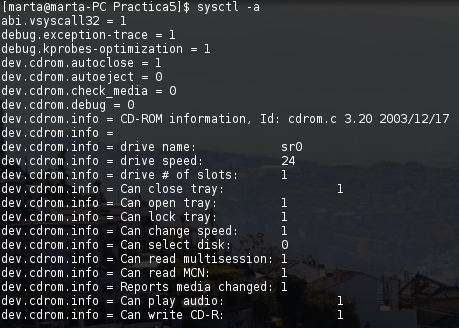
\includegraphics[width=0.5\textwidth]{1}
    \caption{Parte del output obtenido al ejecutar \texttt{sysctl -a}}
    \label{sysctla}
\end{figure}

Tal y como se dice en \cite{archsysctl}, si tenemos el paquete \texttt{linux-docs} instalado podremos acceder a información detallada de cada módulo en \texttt{/proc/sys}. Dicha información se encuentra, en mi caso, en el directorio \texttt{/usr/lib/modules/4.3.3-2-ARCH/build/Documentation/sysctl}. 

Los parámetros de \texttt{sysctl} que he elegido para explicar son:
\begin{enumerate}[---]
    \item \texttt{kernel.shmall}: este parámetro establece la cantidad total de páginas de memoria compartida que se puede usar en todo el sistema.
    \item \texttt{kernel.threads-max}: este parámetro establece el número máximo de hebras que pueden crearse usando \texttt{fork()}.
\end{enumerate}

\section{Realice una copia de seguridad del registro de Windows y restaurela, ilustre el proceso con capturas de pantalla.}
Antes de empezar, debemos instalar el programa \textit{Copias de Seguridad de Windows Server} a través del \textbf{Asistente para agregar características}.

Una vez instalado, seguimos los siguientes pasos para hacer la copia de seguridad:
\begin{enumerate}[1.]
    \item Seguimos la ruta que se ve en la \hyperref[copiaseg]{Figura \ref*{copiaseg}}: \textbf{Inicio $>$ Herramientas administrativas $>$ Copias de seguridad de Windows}.

    \begin{figure}[!h]
        \centering
        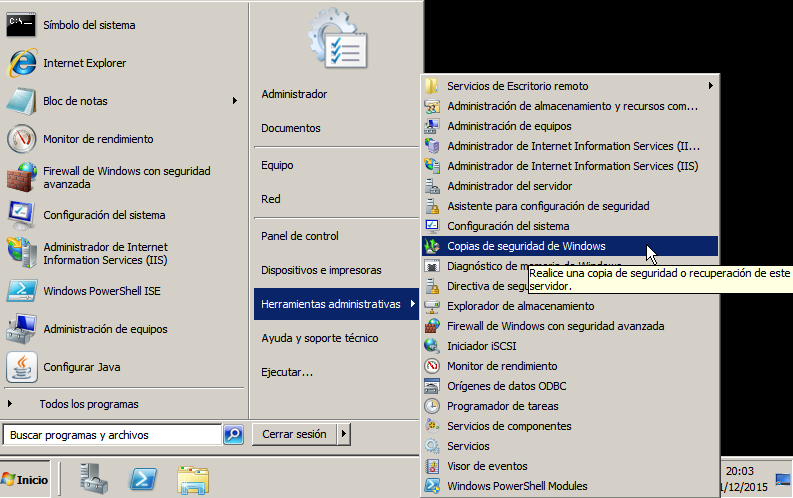
\includegraphics[width=0.7\textwidth]{2}
        \caption{Ruta para ejecutar el programa \textit{Copias de Seguridad de Windows Server}}
        \label{copiaseg}
    \end{figure}

    \item Una vez dentro del programa, seguimos la ruta que se ve en la \hyperref[unavez]{Figura \ref*{unavez}}: \textbf{Acción $>$ Hacer copia de seguridad una vez...}
    \begin{figure}[!h]
        \centering
        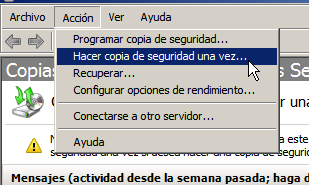
\includegraphics[width=0.5\textwidth]{3}
        \caption{Ruta para hacer una copia de seguridad}
        \label{unavez}
    \end{figure}

    \item Tras esto, accederemos al \textit{Asistente para hacer una copia de seguridad una vez}. En el primer paso, debemos elegir con qué crear la copia de seguridad, en nuestro caso elegimos \textbf{Opciones diferentes}, ya que no hemos creado ninguna copia de seguridad programada (\hyperref[primerpasocopiaseg]{Figura \ref*{primerpasocopiaseg}}).

    \begin{figure}[!h]
        \centering
        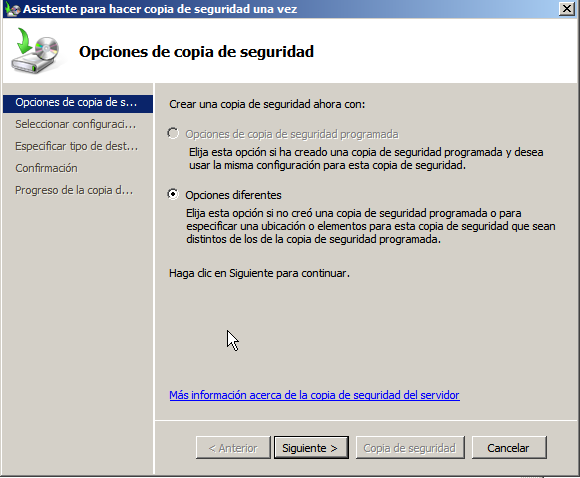
\includegraphics[width=0.5\textwidth]{4}
        \caption{Eligiendo cómo hacer la copia de seguridad}
        \label{primerpasocopiaseg}
    \end{figure}

    \item Después, deberemos elegir qué tipo de configuración programar: si hacer una copia de seguridad de todos los datos o sólo de una parte. En nuestro caso elegiremos la opción \textbf{Personalizada} (\hyperref[segundopasocopiaseg]{Figura \ref*{segundopasocopiaseg}}).

    \begin{figure}[!h]
        \centering
        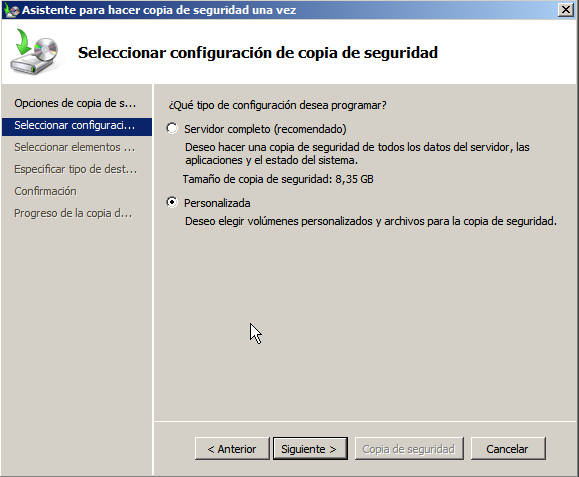
\includegraphics[width=0.5\textwidth]{5}
        \caption{Eligiendo qué configuración programar para la copia de seguridad}
        \label{segundopasocopiaseg}
    \end{figure}

    \item A continuación, elegiremos qué incluir en la copia de seguridad. En nuestro caso únicamente incluiremos el \textbf{Estado del Sistema} (\hyperref[tercerpasocopiaseg]{Figura \ref*{tercerpasocopiaseg}}).

    \begin{figure}[!h]
        \centering
        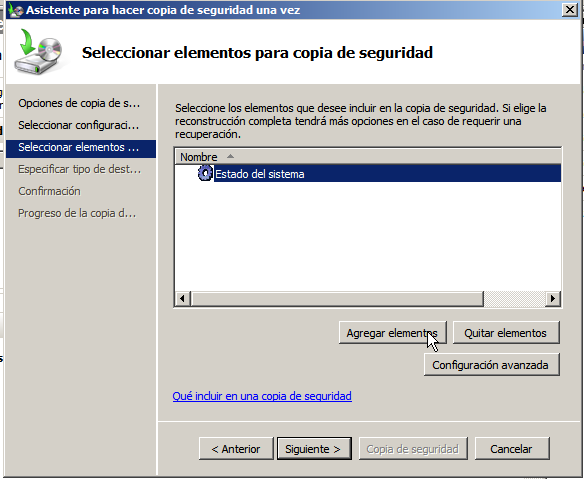
\includegraphics[width=0.5\textwidth]{6}
        \caption{Seleccionando los elementos a incluir en la copia de seguridad}
        \label{tercerpasocopiaseg}
    \end{figure}

    \item Posteriormente, seleccionamos el tipo de almacenamiento en el que guardaremos la copia de seguridad, en nuestro caso, \textbf{Unidades locales} (\hyperref[cuartopasocopiaseg]{Figura \ref*{cuartopasocopiaseg}}).

    \begin{figure}[!h]
        \centering
        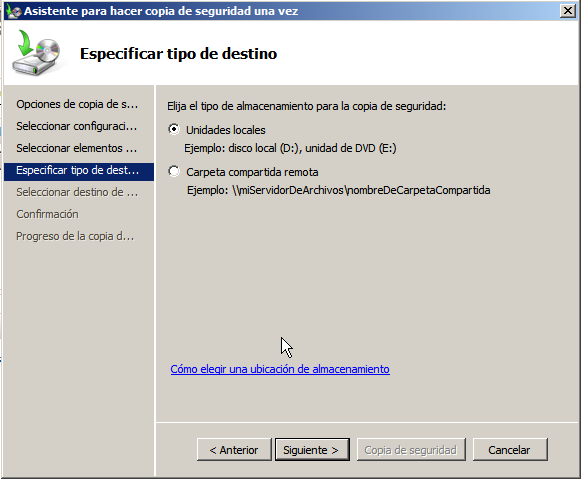
\includegraphics[width=0.5\textwidth]{7}
        \caption{Seleccionando el tipo de almacenamiento en el que guardar la copia de seguridad}
        \label{cuartopasocopiaseg}
    \end{figure}

    \item Tras esto, seleccionamos el dispositivo en el que almacenaremos nuestra copia de seguridad, en nuestro caso seleccionaremos la unidad D (\hyperref[quintopasocopiaseg]{Figura \ref*{quintopasocopiaseg}}).

    \begin{figure}[!h]
        \centering
        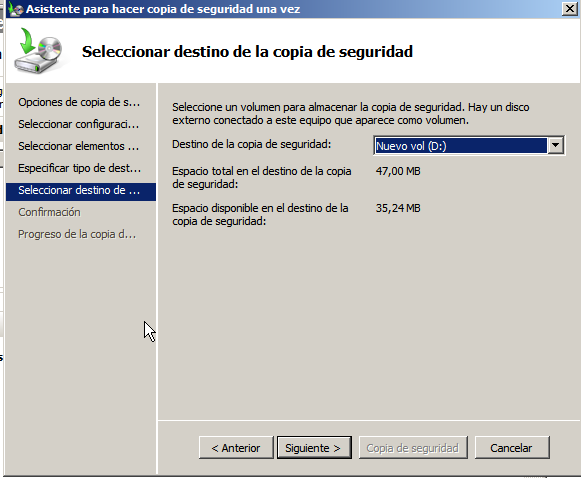
\includegraphics[width=0.5\textwidth]{8}
        \caption{Seleccionando dónde guardar la copia de seguridad}
        \label{quintopasocopiaseg}
    \end{figure}

    \item Por último, confirmamos todos los pasos anteriores y hacemos click en \textbf{Copia de Seguridad}.

    \begin{figure}[!h]
        \centering
        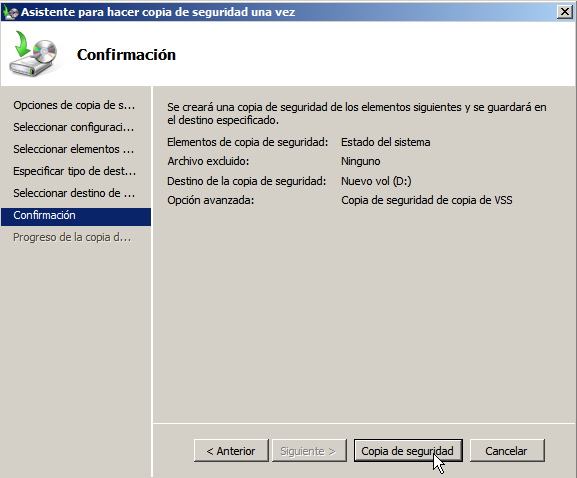
\includegraphics[width=0.5\textwidth]{9}
        \caption{Confirmando todos los pasos del asistente}
        \label{sextopasocopiaseg}
    \end{figure}

    \item Si todo ha salido bien, veremos una ventana como la de la \hyperref[copiasegestadosis]{Figura \ref*{copiasegestadosis}}.

    \begin{figure}[!h]
        \centering
        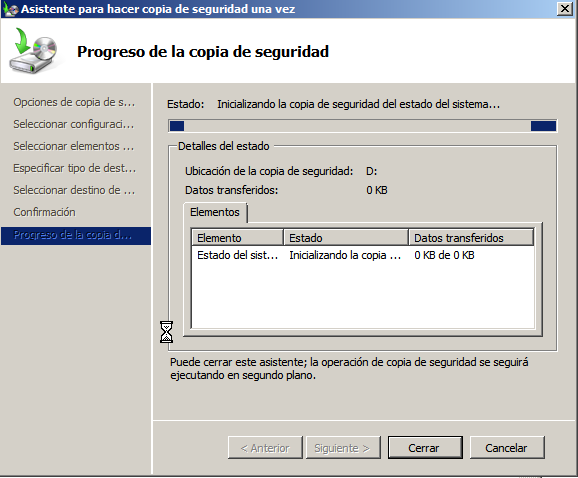
\includegraphics[width=0.5\textwidth]{10}
        \caption{Haciendo la copia de seguridad del estado del sistema}
        \label{copiasegestadosis}
    \end{figure}
\end{enumerate}

Una vez hecha la copia de seguridad, para restaurar el registro hay que seguir los siguientes pasos:
\begin{enumerate}[1.]
\item Abrimos el programa \textbf{Copias de seguridad de Windows}, tal y como hicimos antes (\hyperref[copiaseg]{Figura \ref*{copiaseg}}).
\item Seguimos la ruta \textbf{Acción $>$ Recuperar...} (\hyperref[recuperar]{Figura \ref*{recuperar}}).
    \begin{figure}[!h]
        \centering
        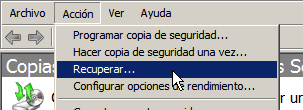
\includegraphics[width=0.5\textwidth]{11}
        \caption{Ruta para ejecutar el asistente de recuperación a partir de una copia de seguridad}
        \label{recuperar}
    \end{figure}

\item Tras esto, se nos abrirá el \textbf{Asistente para la recuperación}. En primer lugar, debemos seleccionar dónde está almacenada la copia de seguridad que se usará para recuperar. En nuestro caso, seleccionaremos \textbf{En este servidor}. (\hyperref[ubicopy]{Figura \ref*{ubicopy}}).

    \begin{figure}[!h]
        \centering
        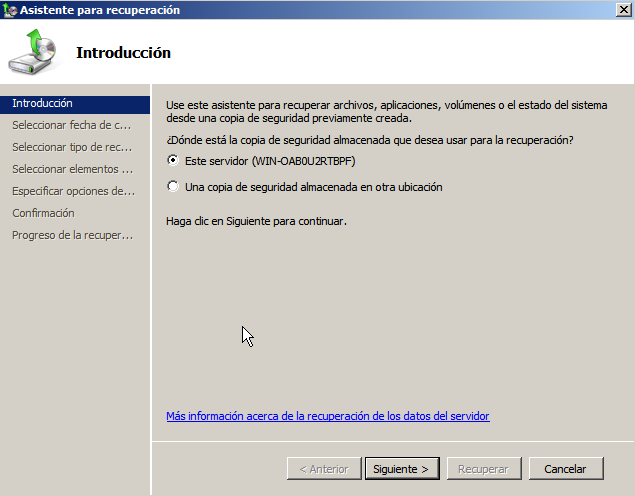
\includegraphics[width=0.5\textwidth]{12}
        \caption{Seleccionando la ubicación de la copia de seguridad que se usará}
        \label{ubicopy}
    \end{figure}

\item A continuación, seleccionamos la fecha en la cual hicimos la copia de seguridad, en este caso el 3 de Enero de 2016 (\hyperref[fechacopy]{Figura \ref*{fechacopy}}).

    \begin{figure}[!h]
        \centering
        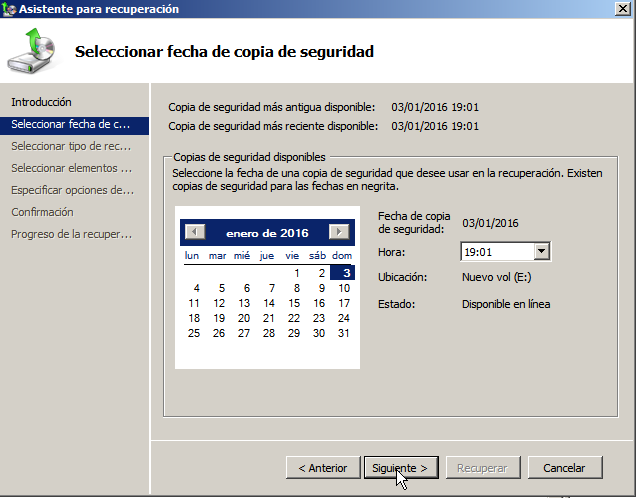
\includegraphics[width=0.5\textwidth]{13}
        \caption{Seleccionando la fecha de la copia de seguridad que se usará}
        \label{fechacopy}
    \end{figure}

\item Después, el asistente nos preguntará dónde queremos realizar la recuperación del sistema, en nuestro caso lo dejamos con la ubicación original (\hyperref[ubires]{Figura \ref*{ubires}}).

    \begin{figure}[!h]
        \centering
        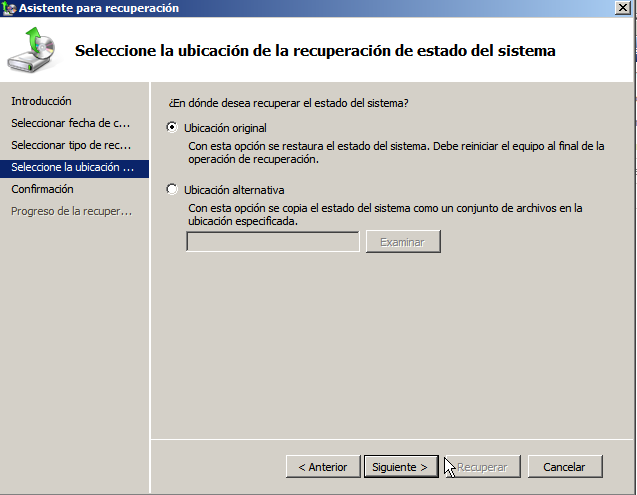
\includegraphics[width=0.5\textwidth]{14}
        \caption{Seleccionando la ubicación de la restauración del sistema}
        \label{ubires}
    \end{figure}

\item Y finalmente, confirmamos todos los pasos realizados haciendo click en \textbf{Restaurar} y aceptamos el aviso que nos aparece (\hyperref[finres]{Figura \ref*{finres}}).

    \begin{figure}[!h]
    \centering
    \mbox {
    \subfigure[Confirmando todos los ajustes establecidos en el asistente para la restauración]{
    \label{confres}
    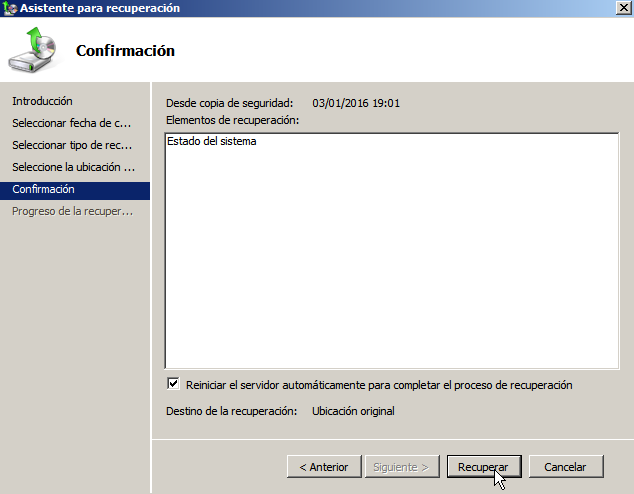
\includegraphics[width=0.5\textwidth]{15}
    }
    \qquad
    \subfigure[Aviso que nos hace el asistente antes de realizar la restauración] {
    \label{avisores}
    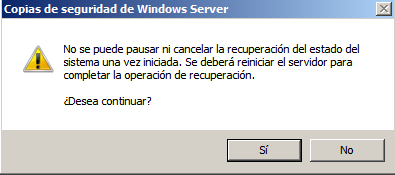
\includegraphics[width=0.5\textwidth]{16}
    }
    }
    \caption{Finalizando la restauración del sistema}
    \label{finres}
    \end{figure}

\item Si todo ha ido bien, veremos la ventana de la \hyperref[ventanares]{Figura \ref*{ventanares}}.

    \begin{figure}[!h]
        \centering
        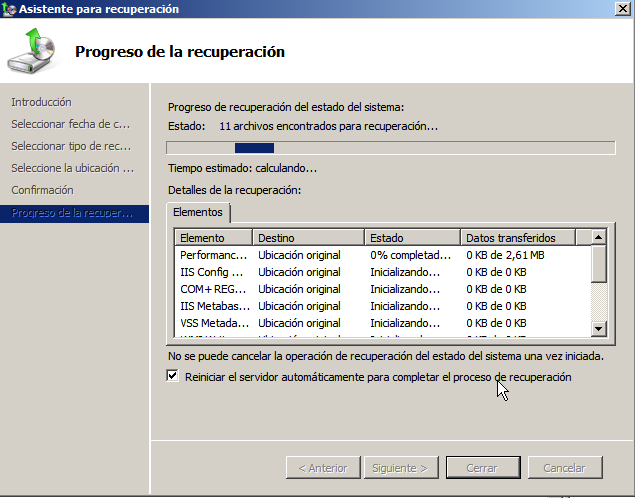
\includegraphics[width=0.5\textwidth]{17}
        \caption{Ventana de progreso de la restauración del sistema}
        \label{ventanares}
    \end{figure}

\item Tras esto, el equipo se reiniciará y veremos el mensaje de la \hyperref[exitores]{Figura \ref*{exitores}}.

    \begin{figure}[!h]
        \centering
        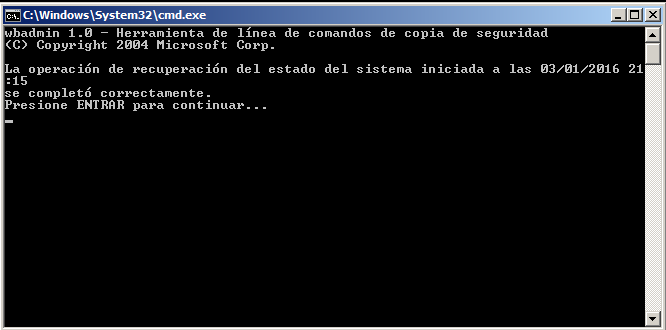
\includegraphics[width=0.5\textwidth]{18}
        \caption{Mensaje de éxito tras reiniciarse el equipo al hacer la restauración}
        \label{exitores}
    \end{figure}

\end{enumerate}

\section{¿Cómo se abre una consola en Windows? ¿Qué comando hay que ejecutar para editar el registro? Muestre su ejecución con capturas de pantalla.}
La consola en windows es un programa llamado \textbf{Símbolo del sistema}, aunque también podemos encontrarlo como \texttt{cmd.exe}. El editor de registro se ejecuta con un comando llamado \texttt{regedit} (\cite{regedit}) (\hyperref[cmd]{Figura \ref*{cmd}}).

\begin{figure}[!h]
    \centering
    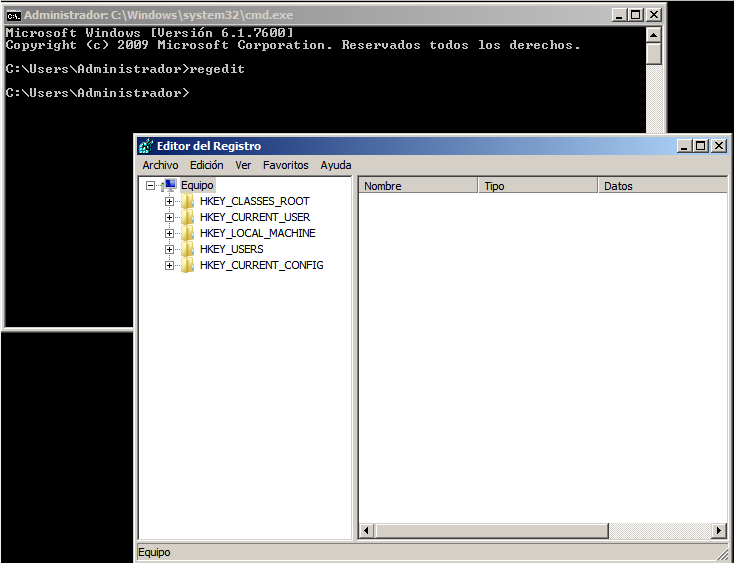
\includegraphics[width=0.7\textwidth]{19}
    \caption{Símbolo del sistema en windows con la orden \texttt{regedit} escrita y la ventana del Editor de Registro}
    \label{cmd}
\end{figure}

\section{Las cadenas de caracteres y valores numéricos del Editor de Registro tienen distintos tipos. Busque en la documentación de Microsoft y liste todos los tipos de valores.}
Según \cite{regtypes}, los distintos tipos de tipos que tienen las cadenas de caracteres y valores numéricos en el Editor de Registro son:
\begin{enumerate}[$\bullet$]
    \item \texttt{REG\_BINARY}: datos binarios guardados en cualquier forma.
    \item \texttt{REG\_DWORD}: un número de 32 bits.
    \item \texttt{REG\_DWORD\_LIITLE\_ENDIAN}: un número de 32 bits en formato \textit{Little Endian}. Windows se ha diseñado para ejecutarse en arquitecturas \textit{Little Endian}, por tanto, este valor está definido como \texttt{REG\_DWORD} en los archivos de cabecera de Windows.
    \item \texttt{REG\_DWORD\_BIG\_ENDIAN}: un número de 32 bits almacenado en formato \textit{Big Endian}.
    \item \texttt{REG\_EXPAND\_SZ}: un string terminado en \texttt{NULL} que contiene punteros a variables de entorno (por ejemplo ``\texttt{\%PATH\%}''). Puede ser \textit{Unicode} o \textit{ANSI} dependiendo de si usamos funciones en \textit{Unicode} o en \textit{ANSI}.
    \item \texttt{REG\_LINK}: un string \textit{Unicode} terminado en \texttt{NULL} que contene la ruta de un enlace símbolico creado con la función \texttt{RegCreateKeyEx} con \texttt{REG\_OPTION\_CREATE\_LINK}.
    \item \texttt{REG\_MULTI\_SZ}:  una secuencia de strings terminados en \texttt{NULL}, terminada con el string vacío ($\backslash0$).
    \item \texttt{REG\_NONE}: tipo sin definir.
    \item \texttt{REG\_QWORD}: un número de 64 bits.
    \item \texttt{REG\_QWORD\_LITTLE\_ENDIAN}: un número de 64 bits en formato \textit{Little Endian}. Al igual que antes, este valor está definido como \texttt{REG\_QWORD} en los archivos de cabecera de Windows.
    \item \texttt{REG\_SZ}: un string terminado en \texttt{NULL}. Puede ser tanto \textit{Unicode} como \textit{ANSI}, dependiendo de si usamos funciones \textit{Unicode} o \textit{ANSI}.
\end{enumerate}

\section{Enumere qué elementos se pueden configurar en Apache y en IIS para que Moodle funcione mejor.}
En \cite{moodle} se enumeran algunos parámetros configurables de Moodle para funcionar mejora tanto en Apache como en IIS.

\subsection{Apache}
Las opciones configurables en Apache más destacadas para aumentar el rendimiento de Moodle son:

\begin{enumerate}[$\bullet$]
    \item Establecer el número máximo de clientes (parámetro \texttt{MaxClients}) al 80\% de la memoria disponible para poder dejar un margen.
    \item Reducir el número de módulos que Apache carga en el fichero \textit{httpd.conf} al mínimo necesario para reducir la memoria necesaria.
    \item Usar la última versión de Apache.
    \item Disminuir el parámetro \texttt{MaxRequestPerChild} en \textit{httpd.conf} hasta un mínimo de 20-30 (Sólo en sistemas Linux/Unix).
    \item Establecer el parámetro \texttt{KeepAlive Off} o disminuir el parámetro \texttt{KeepAliveTimeout} entre 2 y 5.
    \item Si no se usa un fichero \texttt{.htaccess}, establecer la variable \texttt{AllowOverride} a \texttt{None}.
    \item Establecer el \texttt{DirectoryIndex} de forma correcta para poder evitar negociación de contenido.
    \item Establecer \texttt{ExtendedStatus} a \texttt{Off} y desactivar tanto \texttt{mod\_info} como \texttt{mod\_status}
    \item Dejar \texttt{HostnameLookups} a su valor por defecto, \texttt{Off}.
    \item Reducir el valor de \texttt{TimeOut} a entre 30 y 60 segundos.
\end{enumerate}

\subsection{IIS}
En el caso de IIS, deben hacerse la localización del registro \texttt{HKLM$\backslash$ SYSTEM$\backslash$ CurrentControlSet$\backslash$ Services$\backslash$ Inetinfo$\backslash$ Parameters$\backslash$ }. Las opciones más destacables son:
\begin{enumerate}[$\bullet$]
    \item El equivalente a \texttt{KeepAliveTimeout} es \texttt{ListenBackLog} y se debe establecer entre 2 y 5.
    \item Cambiar el valor \texttt{MemCacheSize} para ajustar la cantidad de memoria (en Mb) que IIS usará para su archivo de cache.
    \item Crear un nuevo \texttt{DWORD} llamado \texttt{ObjectCacheTTL} para cambiar cuánto tiempo (en ms) se guardarán los ojetos en memoria.
\end{enumerate}

\section{Ajuste la compresión en el servidor IIS y analice su comportamiento usando varios valores para el tamaño de archivo a partir del cual comprimir. Para comprobar que está comprimiendo puede usar el navegador o comandos como \texttt{curl} o \texttt{lynx}. Muestre capturas de pantalla de todo el proceso.}
\subsection{Configurando el tamaño de compresión}
En \cite{compiis} se explica el proceso para habilitar la compresión HTTP tanto en el servidor como en la página web. Para configurar la compresión en el servidor seguimos los siguientes pasos:
\begin{enumerate}[1.]
    \item Seguimos la ruta que se ve en la \hyperref[rutamaniis]{Figura \ref*{rutamaniis}}: \textbf{Inicio $>$ Herramientas Administrativas $>$ Administrador de Internet Information Services (IIS)}
    \begin{figure}[!h]
        \centering
        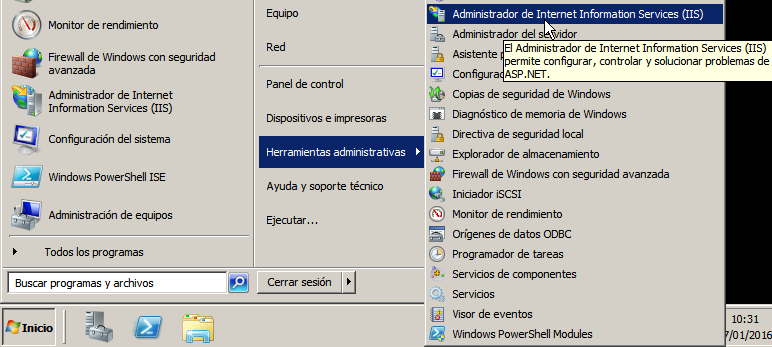
\includegraphics[width=0.5\textwidth]{20}
        \caption{Ruta para acceder al administrador de IIS}
        \label{rutamaniis}
    \end{figure}

    \item Una vez ahí, seleccionamos nuestro servidor y, en el panel de características, buscamos \textbf{Compresión} (\hyperref[searchcomp]{Figura \ref*{searchcomp}}).
    \begin{figure}[!h]
        \centering
        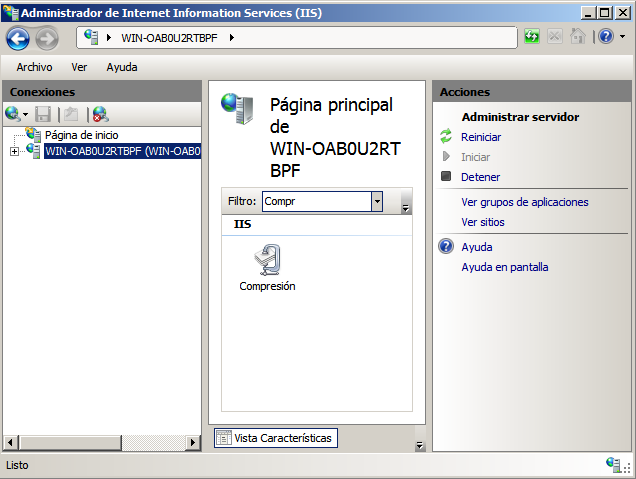
\includegraphics[width=0.5\textwidth]{21}
        \caption{Buscando la utilidad de \textit{Compresión} en el panel de administración de IIS}
        \label{searchcomp}
    \end{figure}

    \item Configuramos el tamaño a partir del cual comprimir y hacemos click en \textbf{Aplicar} (\hyperref[confcompiis]{Figura \ref*{confcompiis}}).
    \begin{figure}[!h]
        \centering
        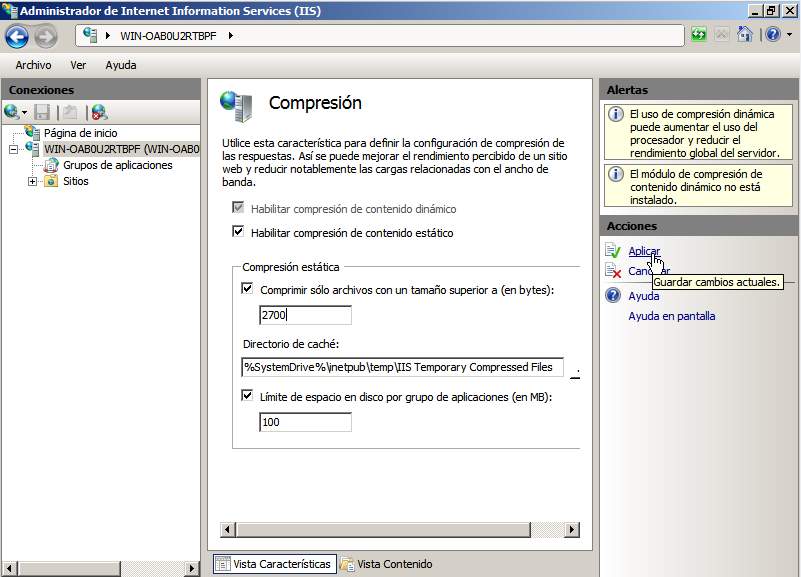
\includegraphics[width=0.5\textwidth]{22}
        \caption{Configurando la compresión en IIS}
        \label{confcompiis}
    \end{figure}
\end{enumerate}

\subsection{Comprobación de la compresión}
Para comprobar la compresión usaremos la consola web que incluye navegador \textit{Mozilla Firefox}, si realmente el servidor ha realizado una compresión, en las cabeceras de la respuesta que podemos ver en la pestaña de red, debemos ver que aparece \textbf{gzip} en el apartado \textbf{Accept-Encoding}, tal y como se aprecia en la \hyperref[comprcompr]{Figura \ref*{comprcompr}}.

\begin{figure}[!h]
    \centering
    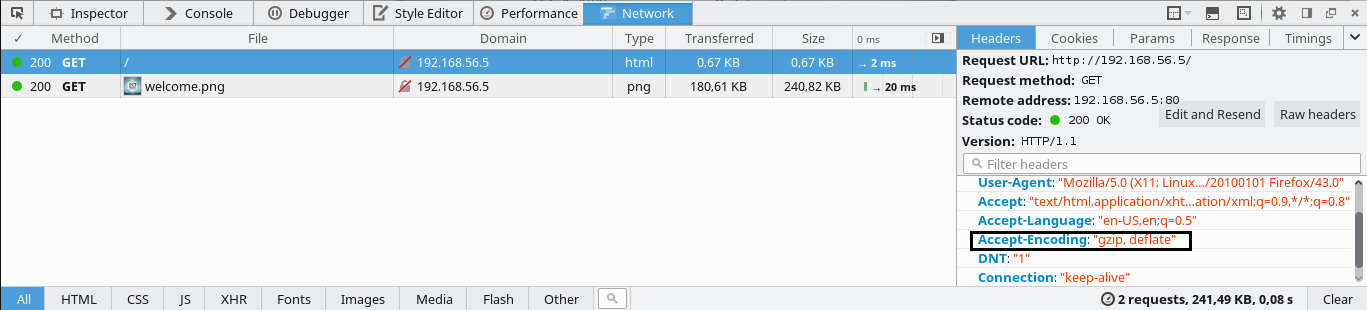
\includegraphics[width=1\textwidth]{26}
    \caption{Comprobación de que, efectivamente, el servidor ha realizado una compresión}
    \label{comprcompr}
\end{figure}

Tras saber que efectivamente el servidor está comprimiendo los archivos mayores a un determinado tamaño, hemos probado tres tamaños distintos de compresión:
\begin{enumerate}[$\bullet$]
    \item En primer lugar, hemos probado el valor de compresión por defecto de IIS, \textbf{2700 Bytes}, y hemos obtenido el resultado que se ve en la \hyperref[compr1]{Figura \ref*{compr1}}: 10ms para transferir el archivo HTML y 13, para transferir la imagen, cuyo tamaño es mayor al de compresión.

    \begin{figure}[!h]
        \centering
        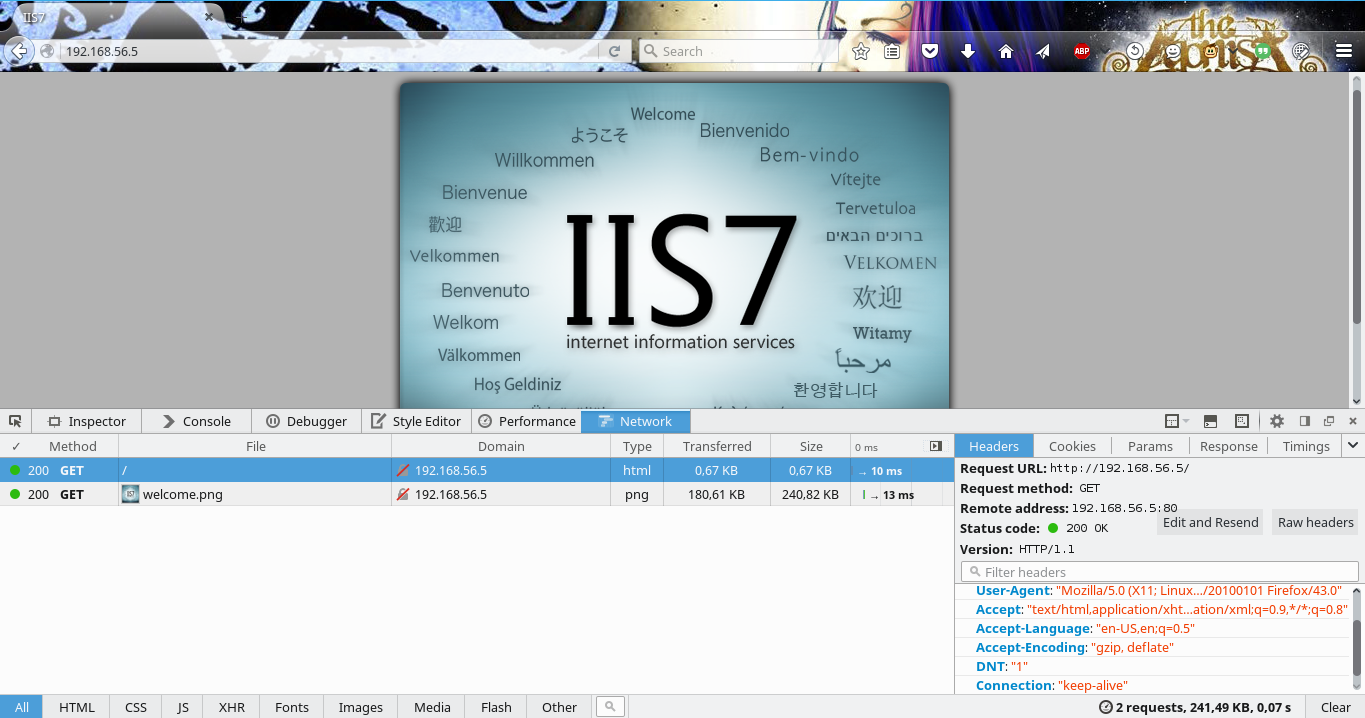
\includegraphics[width=0.8\textwidth]{23}
        \caption{Tiempo que ha tardado el servidor en enviar los archivos con un tamaño de compresión de 2700 Bytes}
        \label{compr1}
    \end{figure}

    \item Después, hemos probado un valor menor al tamaño del documento HTML, \textbf{500 Bytes} de compresión, y hemos obtenido el resultado que se ve en la \hyperref[compr2]{Figura \ref*{compr2}}: 1ms para transferir el archivo HTML y 60, para transferir la imagen.

    \begin{figure}[!h]
        \centering
        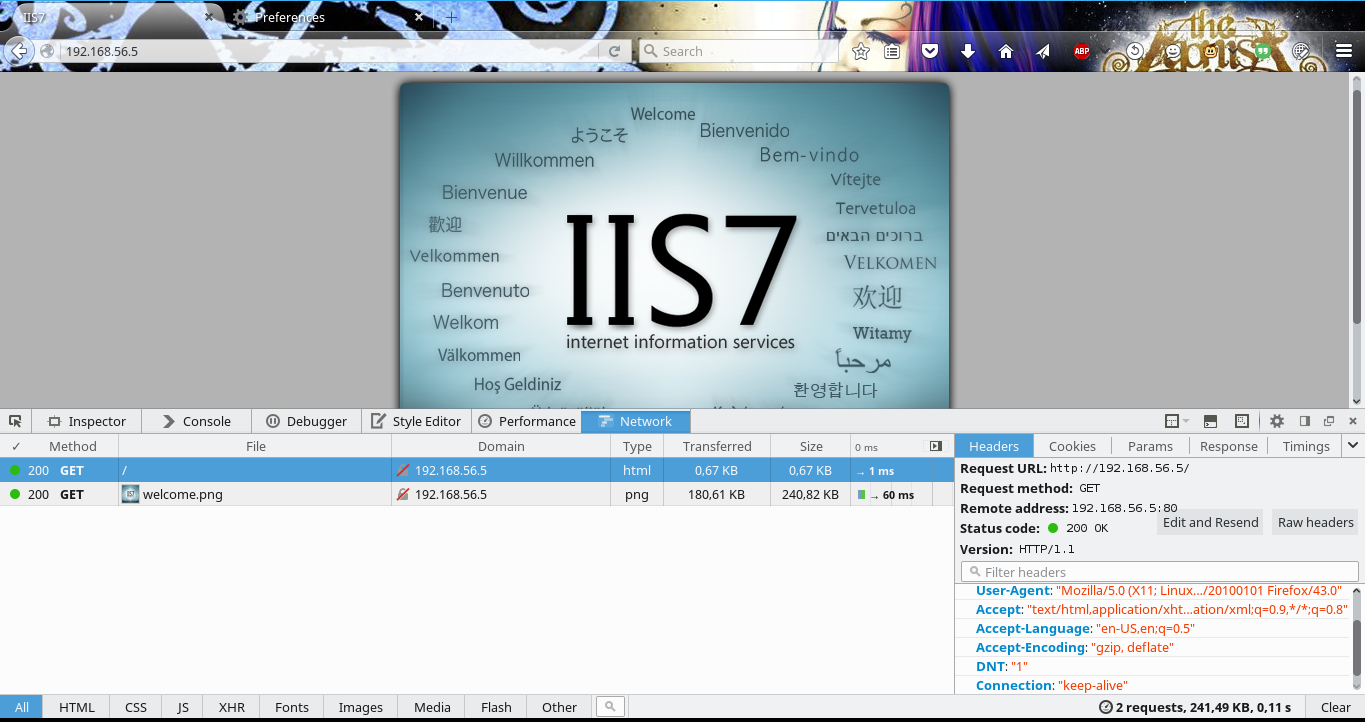
\includegraphics[width=0.8\textwidth]{24}
        \caption{Tiempo que ha tardado el servidor en enviar los archivos con un tamaño de compresión de 500 Bytes}
        \label{compr2}
    \end{figure}

    \item Y por último, hemos probado un valor mayor al tamaño de la imagen, \textbf{256000 Bytes}, y hemos obtenido el resultado que se ve en la \hyperref[compr3]{Figura \ref*{compr3}}: 8ms para transferir el archivo HTML y 95, para transferir la imagen.

        \begin{figure}[!h]
            \centering
            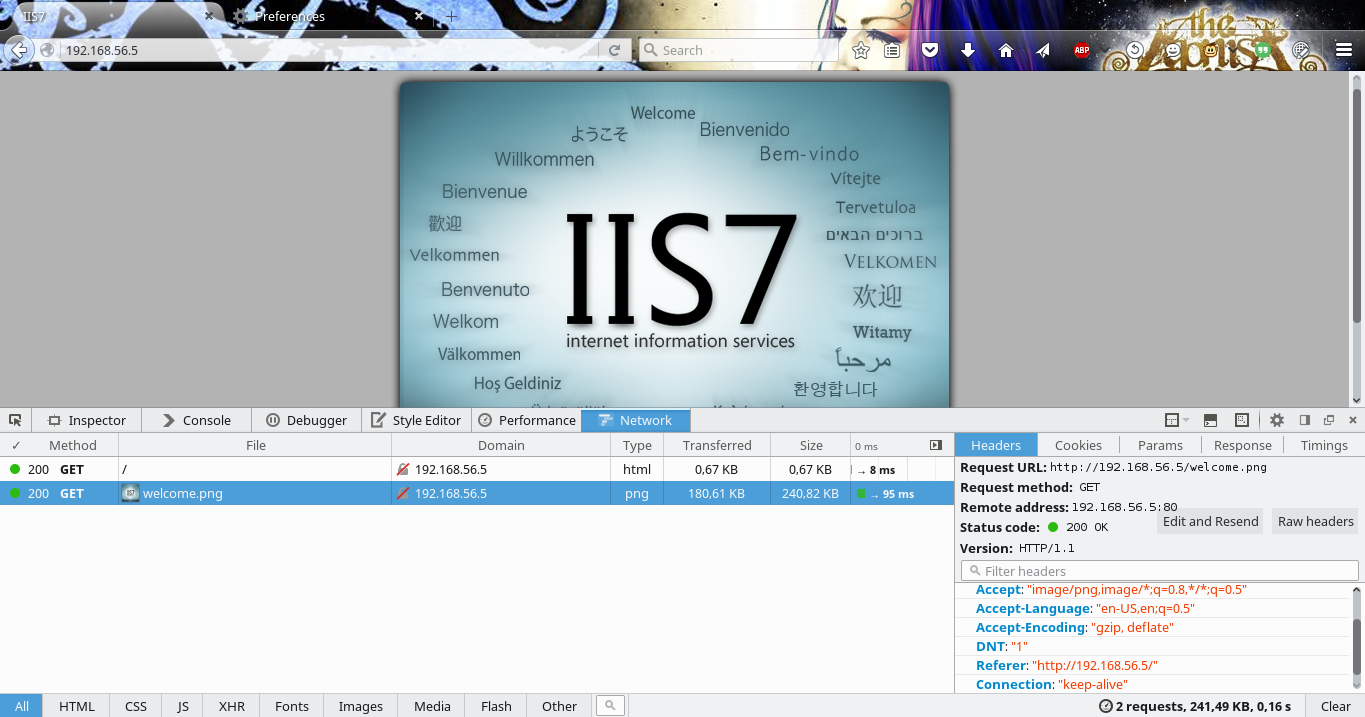
\includegraphics[width=0.8\textwidth]{25}
            \caption{Tiempo que ha tardado el servidor en enviar los archivos con un tamaño de compresión de 256000 Bytes}
            \label{compr3}
        \end{figure}
\end{enumerate}

Por tanto, podemos concluir que la mejor compresión es la que tenía IIS por defecto, \textbf{2700 Bytes}. Ya que es con la que conseguimos la mejor relación de tiempo entre la imagen y el archivo HTML.

\section{Usted parte de un sistema operativo con ciertos parámetros definidos en la instalación (Práctica 1), ya sabe instalar servicios (Práctica 2) y cómo monitorizarlos (Práctica 3) cuando los somete a cargas (Práctica 4). Al igual que ha visto cómo se puede mejorar un servidor web (Práctica 5 Sección 3.1), elija un servicio (el que usted quiera) y modifique un parámetro para mejorar su comportamiento. Monitorice el servicio antes y después de la modificación del parámetro aplicando cargas al sistema (antes y después) mostrando los resultados de la monitorización.}
% Sugerencia de Alberto: asumiento un servicio de almacenamiento basado en ubuntu 15 y sistemas de archivos encriptados, ampliar el tamaño de los discos.
Ofrecemos un servicio de almacenamiento en un servidor con sistema operativo Ubuntu 15.05. Almacenamos los datos de los usuarios en una partición encriptada con \textbf{LUKS}. El espacio libre en dicha partición está empezando a agotarse, por lo que sería preciso incrementar su espacio libre (\hyperref[antes]{Figura \ref*{antes}}).

\begin{figure}[!h]
    \centering
    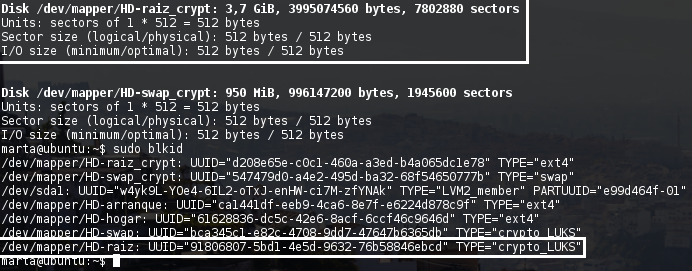
\includegraphics[width=0.7\textwidth]{27}
    \caption{Características del sistema de archivos \texttt{HD-raiz}, antes de incrementar su capacidad, comprobado usando los comandos \texttt{fdisk} (\cite{fdisk}) y \texttt{blkid} (\cite{blkid})}
    \label{antes}
\end{figure}

Los pasos a seguir son:
\begin{enumerate}[1.]
    \item Arrancamos con el live CD de Ubuntu y hacemos click en \textbf{Probar Ubuntu} (\hyperref[instalador]{Figura \ref*{instalador}}).
\begin{figure}[!h]
    \centering
    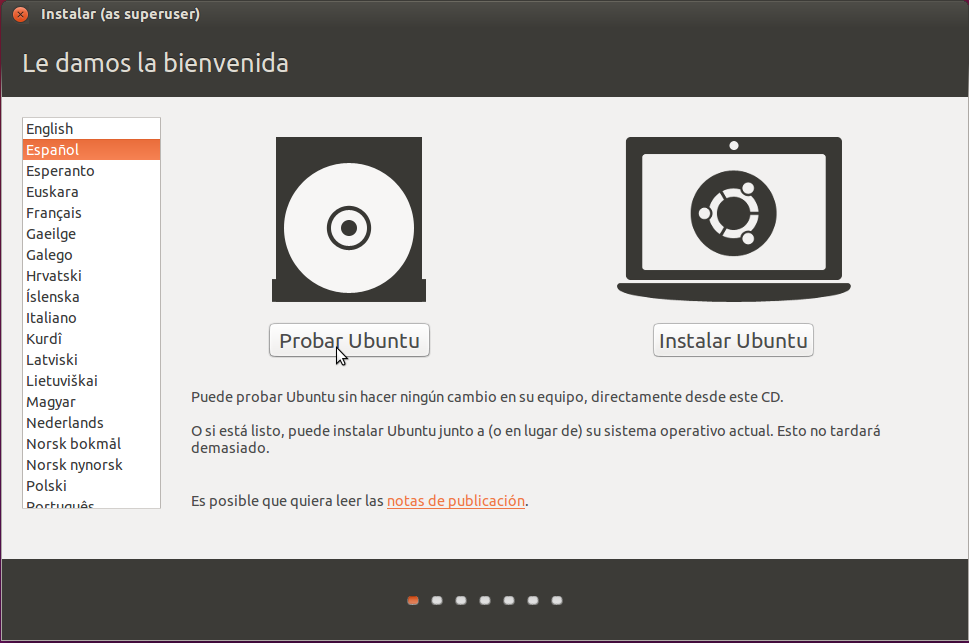
\includegraphics[width=0.5\textwidth]{28}
    \caption{Pantalla de bienvenida al instalador de Ubuntu}
    \label{instalador}
\end{figure}

    \item Una vez nos apareza el escritorio de Ubuntu, abrimos una terminal (\hyperref[terminal]{Figura \ref*{terminal}}).

\begin{figure}[!h]
    \centering
    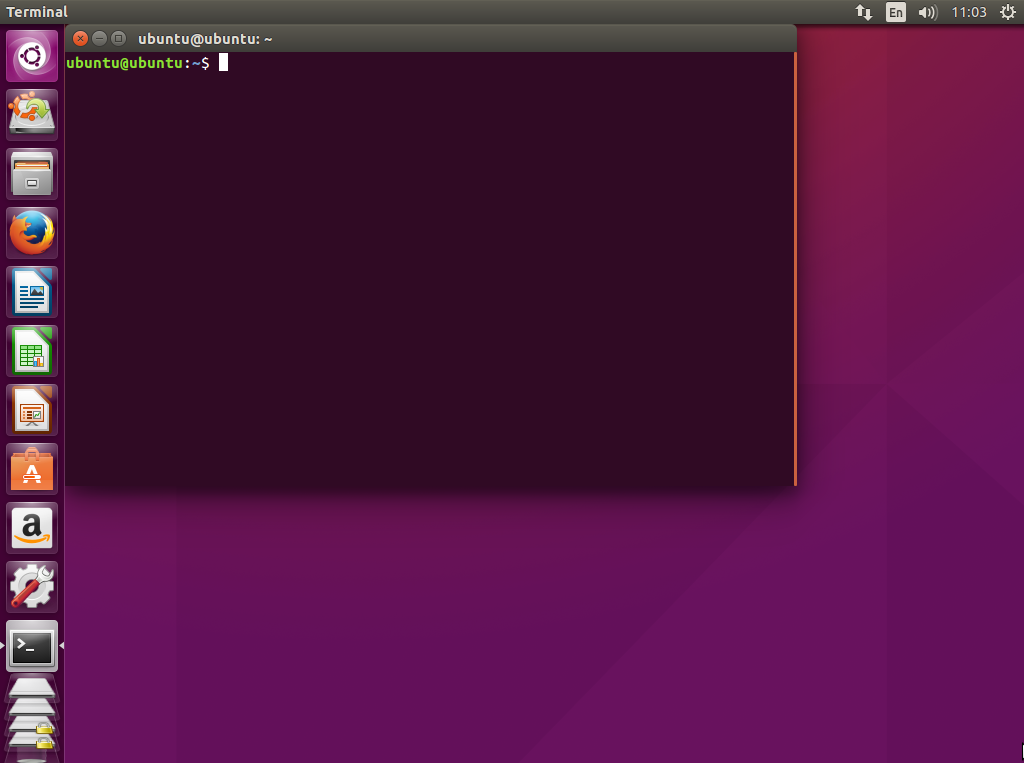
\includegraphics[width=0.5\textwidth]{29}
    \caption{Escritorio de Ubuntu con una terminal abierta}
    \label{terminal}
\end{figure}

    \item Descargamos los paquetes \texttt{lvm2} y \texttt{cryptsetup}:
\begin{minted}[frame=single, label={Descargando lvm2 y cryptsetup}]{bash}
sudo apt-get update && sudo apt-get install lvm2 cryptsetup    
\end{minted}
    \item Cargamos el módulo \texttt{cryptsetup} con \texttt{modprobe} (\cite{modprobe}):
\begin{minted}[frame=single, label={Cargando el módulo cryptsetup}]{bash}
sudo modprobe dm-crypt
\end{minted}
    \item Desencriptamos el sistema de archivos deseado, en nuestro caso se llama \textit{raiz} (\cite{cryptsetup}):
\begin{minted}[frame=single, label={Desencriptando el sistema de archivos HD-raiz}]{bash}
sudo cryptsetup luksOpen /dev/mapper/HD-raiz crypt1
\end{minted}

    En este paso es donde se aprecia la necesidad de usar el live CD, ya que necesitamos que el sistema de archivos en cuestión no esté montado para poder manipularlo. Cuando nos pida una contraseña, deberemos introducir la contraseña para desbloquear dicho sistema de archivos.

    \item Reconocemos todos los grupos de volúmenes que hay en nuestro disco con \texttt{vgscan} (\cite{vgscan}):
\begin{minted}[frame=single, label={Reconociendo los volúmenes físicos en disco}]{bash}
sudo vgscan --mknodes
\end{minted}
    \item y reconocemos (o activamos) también los volúmenes lógicos con \texttt{vgchange} (\cite{vgchange}):
\begin{minted}[frame=single, label={Reconociendo los volúmenes lógicos en disco}]{bash}
sudo vgchange -ay
\end{minted}

Llegados a este paso (\hyperref[pasos]{Figura \ref*{pasos}}), ya nos encontramos en disposición de gestionar la partición encriptada \textit{raiz}.

\begin{figure}[!h]
    \centering
    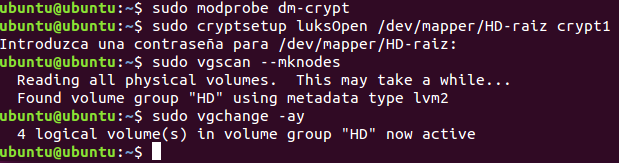
\includegraphics[width=0.65\textwidth]{30}
    \caption{Comandos usados para desencriptar y preparar la partición encriptada}
    \label{pasos}
\end{figure}

\item Incrementamos el tamaño del sistema de archivos, en este caso en 2GB, usando \texttt{lvresize} (\cite{lvresize}):
\begin{minted}[frame=single, label={Incrementando el tamaño del sistema de archivos}]{bash}
sudo lvresize -L +2G /dev/HD/raiz
\end{minted}

\item E incrementamos el tamaño del sistema de archivos encriptado:
\begin{minted}[frame=single, label={Incrementando el tamaño del sistema de archivos encriptado}]{bash}
sudo cryptsetup resize /dev/mapper/HD-raiz
\end{minted}
\end{enumerate}

Tras reiniciar y abrir otra vez la máquina virtual de forma normal, ejecutando el comando \texttt{fdisk -l} vemos, en la \hyperref[finalyay]{Figura \ref*{finalyay}}, que el tamaño del sistema de archivos \textit{raiz} ha incrementado en 2GB.
\begin{figure}[!h]
    \centering
    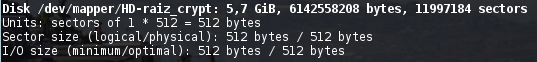
\includegraphics[width=0.55\textwidth]{31}
    \caption{Comprobación final del tamaño del sistema de archivos raiz tras incrementar su tamaño}
    \label{finalyay}
\end{figure}

\begin{figure}[!h]
\centering
\mbox {
\subfigure[Confirmando todos los ajustes establecidos en el asistente para la restauración]{
\label{confres}
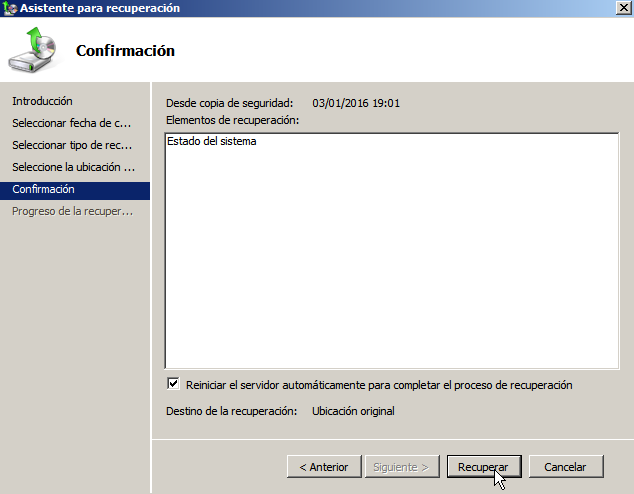
\includegraphics[width=0.5\textwidth]{15}
}
\qquad
\subfigure[Aviso que nos hace el asistente antes de realizar la restauración] {
\label{avisores}
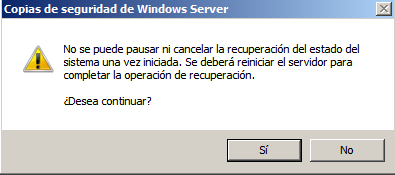
\includegraphics[width=0.5\textwidth]{16}
}
}
\caption{Finalizando la restauración del sistema}
\label{finres}
\end{figure}

% resize2fs

\bibliography{P5-MarGomMac.bib} %archivo citas.bib que contiene las entradas 
\bibliographystyle{siam} % haycle varias formas de citar

\end{document}
